\begin{figure}[h]
    \centering
    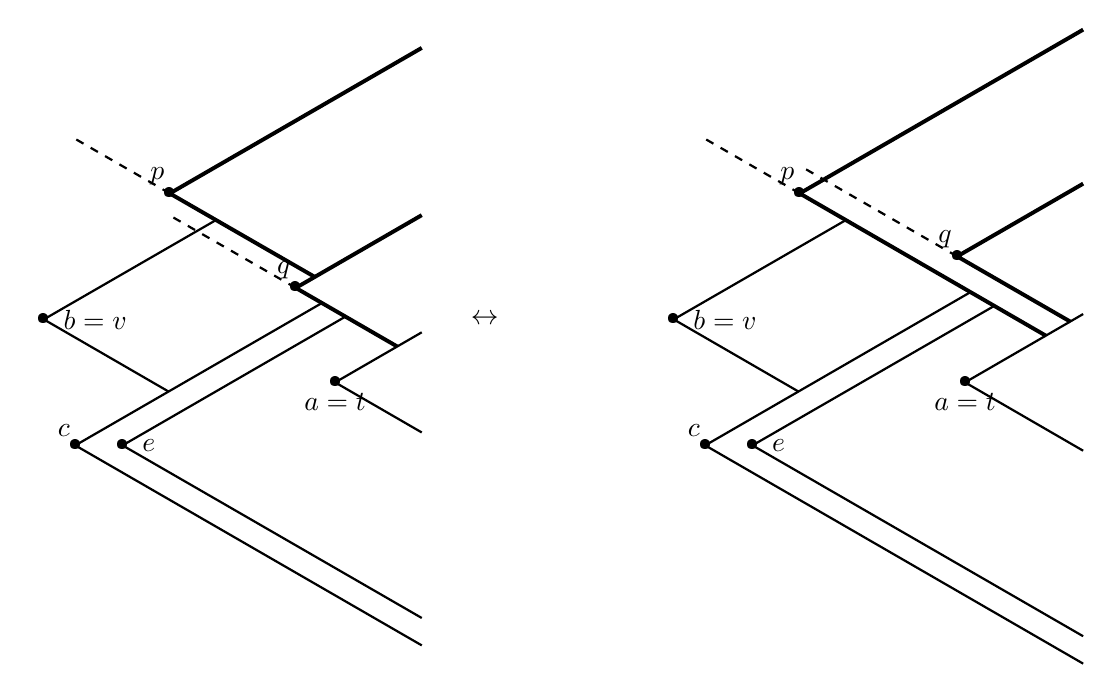
\begin{tikzpicture}[thick, scale=0.4]
        \node[label={[label distance = -3mm]160:$p$}] at
            (2.00, 4.00) {\textbullet};
        \node[label={[label distance = -3mm]160:$q$}] at
            (6.00, 1.00) {\textbullet};
        \node[label={[label distance = -2mm]270:$a = t$}] at
            (7.25, -2.00) {\textbullet};
        \node[label={[label distance = -3mm]160:$c$}] at
            (-1.00, -4.00) {\textbullet};
        \node[label={[label distance = -1mm]0:$b = v$}] at
            (-2.00, 0.00) {\textbullet};
        \node[label={[label distance = -1mm]0:$e$}] at
            (0.50, -4.00) {\textbullet};

        % a cone
        \draw (7.25, -2.00) -- (10.00, -3.59);
        \draw (7.25, -2.00) -- (10.00, -0.41);
        % q cone
        \draw[line width = 0.5mm] (6.00, 1.00) -- (9.22, -0.86);
        \draw[line width = 0.5mm] (6.00, 1.00) -- (10.00, 3.31);
        % p cone
        \draw[line width = 0.5mm] (2.00, 4.00) -- (6.60, 1.35);
        \draw[line width = 0.5mm] (2.00, 4.00) -- (10.00, 8.62);
        % e cone
        \draw (0.50, -4.00) -- (10.00, -9.48);
        \draw (0.50, -4.00) -- (7.58, 0.09);
        % c cone
        \draw (-1.00, -4.00) -- (10.00, -10.35);
        \draw (-1.00, -4.00) -- (6.83, 0.52);
        % b cone
        \draw (-2.00, 0.00) -- (1.96, -2.29);
        \draw (-2.00, 0.00) -- (3.46, 3.15);


        \draw[dashed] (2.00, 4.00) -- (-1.00, 5.73);
        \draw[dashed] (6.00, 1.00) -- (2.00, 3.30);
        \node at (12, 0) {$ \leftrightarrow$};

        \node[label={[label distance = -3mm]160:$p$}] at
            (22.00, 4.00) {\textbullet};
        \node[label={[label distance = -3mm]160:$q$}] at
            (27.00, 2.00) {\textbullet};
        \node[label={[label distance = -2mm]270:$a = t$}] at
            (27.25, -2.00) {\textbullet};
        \node[label={[label distance = -3mm]160:$c$}] at
            (19.00, -4.00) {\textbullet};
        \node[label={[label distance = -1mm]0:$b = v$}] at
            (18.00, 0.00) {\textbullet};
        \node[label={[label distance = -1mm]0:$e$}] at
            (20.50, -4.00) {\textbullet};

        % a cone
        \draw (27.25, -2.00) -- (31.00, -4.17);
        \draw (27.25, -2.00) -- (31.00, 0.17);
        % q cone
        \draw[line width = 0.5mm] (27.00, 2.00) -- (30.59, -0.07);
        \draw[line width = 0.5mm] (27.00, 2.00) -- (31.00, 4.31);
        % p cone
        \draw[line width = 0.5mm] (22.00, 4.00) -- (29.82, -0.52);
        \draw[line width = 0.5mm] (22.00, 4.00) -- (31.00, 9.20);
        % e cone
        \draw (20.50, -4.00) -- (31.00, -10.06);
        \draw (20.50, -4.00) -- (28.18, 0.43);
        % c cone
        \draw (19.00, -4.00) -- (31.00, -10.93);
        \draw (19.00, -4.00) -- (27.43, 0.87);
        % b cone
        \draw (18.00, 0.00) -- (21.96, -2.29);
        \draw (18.00, 0.00) -- (23.46, 3.15);

        \draw[dashed] (22.00, 4.00) -- (19.00, 5.73);
        \draw[dashed] (27.00, 2.00) -- (22.00, 4.88);
    \end{tikzpicture}
    \caption{Da esquerda para a direita,
    todos os pontos de $\Hits_{up}(q)$
    são transferidos para $\Hits_{up}(p)$
    e $p$, que está em $\Hits_{low}(q)$,
    é transferido para $\Hits_{low}(t)$.
    Da direita para esquerda, os pontos
    em $\Hits_{up}(p)$ são transferidos
    para $\Hits_{up}(q)$ e $p$, que está
    em $\Hits_{low}(t)$, é transferido
    para $\Hits_{low}(q)$.}
    \label{fig:parcinetico:eventouptnaoexiste}
\end{figure}